\subsection{Maximizing Whip Performance: The Perfect Spot for Your Loading Coil!}

\begin{tcolorbox}[colback=gray!10, colframe=black, title=E9D03] What is the most efficient location for a loading coil on an electrically short whip? 
\begin{enumerate}[label=\Alph*.]
    \item \textbf{Near the center of the vertical radiator}
    \item As low as possible on the vertical radiator
    \item At a voltage maximum
    \item At a voltage null
\end{enumerate} \end{tcolorbox}

\subsubsection{Explanation of the Concepts}

In radio communications, loading coils are used to electrically lengthen antennas, particularly when dealing with short antennas such as whip antennas. An electrically short whip is one that is significantly less than a half-wavelength in length at the operating frequency. The placement of the loading coil is crucial for maximizing antenna efficiency and performance.

Loading coils create a reactive component that can help match the impedance of the antenna system to that of the transmission line and the feed point. The efficiency and performance of an antenna can be affected by where a loading coil is placed relative to the radiator.

In this context:

- \textbf{Option A: Near the center of the vertical radiator:} is correct because placing the loading coil at this location maximizes the effectiveness of the coil and contributes to a more favorable current distribution along the antenna. This position tends to enhance radiation efficiency and reduce losses.

- \textbf{Option B: As low as possible on the vertical radiator:} does not harness the benefits of the radiation pattern effectively, thus could reduce overall antenna performance.

- \textbf{Option C: At a voltage maximum\textbf{ and }Option D: At a voltage null:} refer to the standing wave pattern of the antenna. While certain configurations in wave antennas might exploit these positions optimally, they are generally not as effective for whip antennas compared to the central position.

\subsubsection{Calculations and Visualization}

For the sake of understanding the current distribution and voltage standing wave ratios (VSWR), we can employ the following relationship for the standing wave amplitude along the antenna:

1. The total length \(L\) of the whip can be expressed in terms of the wavelength \(\lambda\):
   \[
   L = \frac{\lambda}{k}
   \]
   where \(k < 1\) for electrically short antennas.

2. The input impedance \(Z_{in}\) at the feed point is dependent on the positioning:
   \[
   Z_{in} = R + jX
   \]
   where \(R\) is the radiation resistance and \(X\) is the reactance.

3. Analyzing the current (I) distribution across the whip and voltage (V), we can visualize:
   \begin{center}
   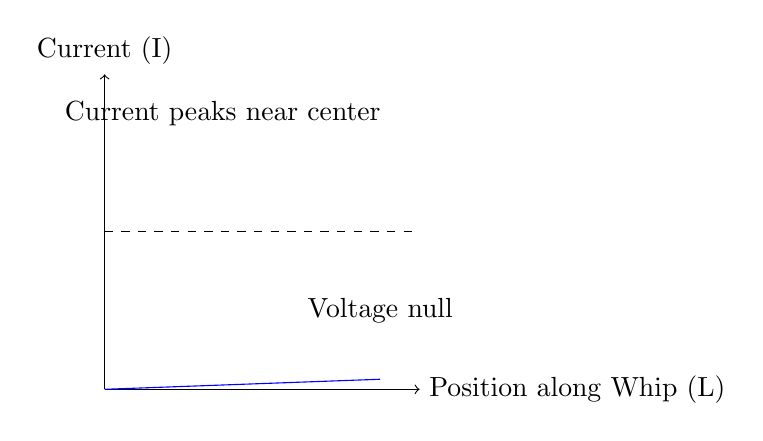
\begin{tikzpicture}
       \draw[->] (0,0) -- (0,4) node[above] {Current (I)};
       \draw[->] (0,0) -- (4,0) node[right] {Position along Whip (L)};
       \draw[domain=0:3.5,smooth,variable=\x,blue] plot ({\x},{2*sin(3.14*\x/3)});
       \draw[dashed] (0,2) -- (4,2);
       \node at (1.5,3.5) {Current peaks near center};
       \node at (3.5,1) {Voltage null};
   \end{tikzpicture}
   \end{center}

This diagram illustrates current distribution along the electrically short whip. It emphasizes the significance of placing the loading coil near the center where the current amplitude is maximized and minimizes losses due to reactance.

In conclusion, positioning the loading coil near the center of the vertical radiator optimizes the performance of the whip antenna by taking advantage of the current distribution characteristics and enhancing radiation efficiency and pattern. Thus, the best answer to the question is \textbf{(A) Near the center of the vertical radiator}. 
